% Chapter 2

\chapter{项目需求分析} % Main chapter title

\label{Chapter2} 
\section{用户背景介绍}
智慧足迹数据科技有限公司是中国联通集团控股,由中国联通和西班牙电信合资成立的专业大数据公司,依托中国联通卓越的数据能力、全球最强大的手机信令处理平台Smart Steps等产品技术和丰富的市场经验,提供位置信息洞察及相关大数据业务。\\
\indent 智慧足迹公司业务主要涵盖两个方面,分为产品平台和行业方案,这两者呈现相辅相成的关系,基于强大的信令数据资源和数据处理能力构建多元化的大数据平台,为不同需求的客户根据其不同的需求从不同的角度分析数据得出个性化的分析结果,从而得到不同行业解决方案。\\
\indent 数据平台分为数据智能平台,数据洞察平台,能力开放平台,数据引擎平台。其中数据智能平台中的统计数据集是基于联通用户的行为轨迹以及属性标签,通过SS平台的脱敏加工后,结合客户需求,实现不同时空、用户属性视角下的数据统计。产品以Excel或者CSV表格的形式对外提供(可选制图与报告配套销售),内容为统计数据集,客户可基于数据结果直接进行问题的研究以及分析决策。产品的主要功能是职住娱的分布、通勤和游憩、全目的的出行、人口动态变化、跨省跨域迁徙等。统计数据API将城市以250M边长的网格均匀覆盖,以接口调用形式访问,提供每一网格(或区域)各维度的人群特征属性,为进一步开展商业洞察、选址分析、指数评估、潜客挖掘提供数据依据。产品功能主要有基础人流数据、人群画像数据、人群流动数据、人群社会属性数据等。\\
\indent 行业方案主要提供一下四个方面的服务,城市规划,政府治理,商企洞察,金融风控。城市规划设计人口分布分析,城市出行分析,城市间跨域迁徙分析,城市产业经济分析等。
\section{用户需求分析}
人口规模和分布一直是城市规划、 城市管理领域关注的核心问题,尤其是在我国城镇化进入下半场, 人才争夺日益激烈的今天。传统的预测模型多是对于规模的预测,而对人口的时空分布关注较少,总
量预测固然意义很大,但空间分布的重要性也不容小觑。 本项目拟利用智慧足迹公司掌握的某区域近1年的手机信令数据,并结合外部网络公开数据,
在标定不同时段人口分布的基础上,构建合适的模型,实现对周、 小时等
空间粒度,乡镇、 网格等时间粒度的人口分布预测,并评估其可靠性,以
期为城市的监测、 预警等精细化管理,以供参考。\\
\indent 总结而言,就是通过历史的人口时空分布数据,来预测未来的人口时空分布。具体说的话,通过北京六环以内,1km网格尺度的分天分小时人口分布数据(历史数据的时间跨度可以拉长到3个月)预测未来一周 相应网格下每天每小时的人口分布。
\section{市场前景分析}
\subsection{信令数据分析相关案例和技术应用场景}
\subsubsection*{手机信令数据的分析价值}
作为城市活动的参与主体,了解人口活动的分布和规律通常是一个城市所有问题的基础。越来越多的城市管理者和规划师已经意识到人作为重要主体在城市中的重要性。而在城市规划中,“人”的监测难度较大,通过传统人口调查的静态获取数据方式很难得到及时的信息。故而,可以提供用户空间位置的手机信令信息让人口移动的实时检测和分析成为可能。
\subsubsection*{手机信令数据商业化的应用场景}
\begin{itemize}
	\item 国外数据使用案例:\\
	美国电信运营商Verizon成立了精准营销部门Precision Marketing Division。该部门提供精准营销洞察(Precision Market Insights),提供商业数据分析服务。如在美国,棒球和篮球比赛是商家最为看中的营销场合,此前在超级碗和NBA的比赛中,Verizon针对观众的来源地进行了精确数据分析,球队得以了解观众对赞助商的喜好等;美国电信运营商Sprint则利用大数据为行业客户提供消费者和市场洞察,包括人口特征、行为特征以及季节性分析等方面。
	\item 国内数据使用案例 \\
	深入了解具有特定偏好的人群的时空分布特征,找到满足目标客群触达(条件)的户外媒体点位。按照智慧足迹标签分类体系(用户自然属性、时空属性、互联网偏好属性等),筛选用户群体,发现目标客群的常驻地(居住、工作等)分布。
\end{itemize}
\subsubsection*{基于大数据的监测和决策支撑服务}
\begin{itemize}
	\item  国外数据使用案例:客流和选址\\
	西班牙电信于2012年10月成立了动态洞察部门DynamicInsights开展大数据业务,为客户提供数据分析打包服务。该部门与市场研究机构GFK进行合作,在英国、巴西推出了首款产品名为智慧足迹(Smart Steps)。智慧足迹基于完全匿名和聚合的移动网络数据,帮助零售商分析顾客来源和各商铺、展位的人流情况以及消费者特征和消费能力,并将洞察结果面向政企客户提供客流分析和零售店选址服务。
	\item 国内数据使用案例:基于大数据的北京城市副中心典型问题研究\\
	项目紧扣北京城市副中心规划、建设和管理的目标与现实问题,旨在采用手机信令、企业、POI、公交一卡通等多源大数据,建立针对北京城市副中心建设发展过程典型问题的指标体系,并从产业、人、交通、房屋和设施五个方向进行归纳、评估、分析,把握问题演变特征、挖掘认识发展规律,为北京城市副中心建设发展提供决策参考。
\end{itemize}
\subsection{智慧足迹和竞争对手分析}
\subsubsection*{智慧足迹历史和发展}
中国联通智慧足迹座位中国位置大数据应用的第一服务商,是中国联通集团控股,由中国联通和西班牙电信合资成立的专业大数据公司,依托中国联通卓越的数据能力、全球最强大的手机信令处理平台Smart Steps等产品技术和丰富的市场经验,提供位置信息洞察及相关大数据业务。智慧足迹在
公司通过“T”型产品战略赋能产业生态,横向开放合作,结合外部智脑综合利用数据,实现数据增值;纵向垂直应用,为行业客户提供全方位服务。城市规划、商企洞察选址、金融位置应用垂直领域取得了领先地位。支撑国家七大部委及重点省市政府,提供200多个城市规划统计数据集服务,市场占有率80\%,成为信令位置数据应用第一服务商。
\subsubsection*{智慧足迹相关竞争对手及对手}
见表格\ref{table:1}
\begin{table}
\centering
\caption{智慧足迹相关竞争对手及对手}
\label{table:1}
\begin{tabular}{p{0.2\columnwidth}|p{0.2\columnwidth}|p{0.2\columnwidth}|p{0.2\columnwidth}}
\hline
\hline
联通智慧足迹 & 上海数慧 & 清华同衡 & 晶众股份\\
\hline
位置大数据应用提供商&大数据在城市规划应用服务商&传统和创新并进的规划设计院&大数据交通应用服务商\\
\hline
\hline
\end{tabular}
\end{table}
\section{数据预处理和分析}
\subsection{数据清洗}
\subsubsection*{确定基站编号与地理位置间的关系}
之所以我们需要得到基站与网格分布的对应关系,是因为每个网格的人口数据不仅是时序的,还与空间分布有关。例如某网格人数的增加与周围网格人数减少相关。前期的数据预处理得到网格分布可能为后续预测提供方便。\\
\indent 原始的基站编号为 wkt 坐标,通过分析原始数据发现基站的编号不是从零开始连续的,说你有一些位置(山地、河流)等没有人流量的数据;而原始的数据只给出了基站编号对应的 wkt 坐标数据,需要处理得到基站编号基站位置分布的关系,如图\ref{fig:2.1}所示。
\begin{figure}[ht]
\centering
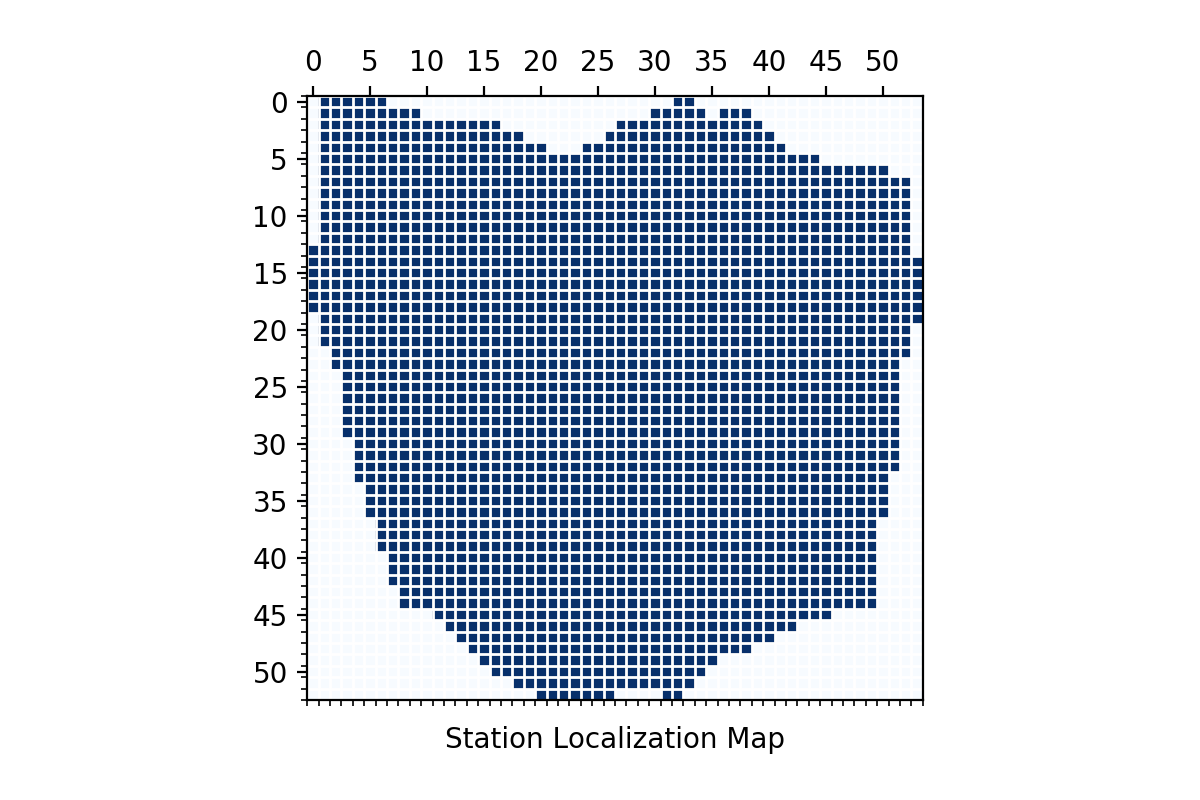
\includegraphics[width=\textwidth]{station_location.png}
\caption{基站位置分布图}
\label{fig:2.1}
\end{figure}
图中显示,基站所覆盖区域被基站划分为54行53列的网格,对应2862个基站,且基站编号从网格左上角开始从左到右从上到下依次加一。图中红色网格代表提供人口流动数据的基站,蓝色网格则是无人区域。\\
\indent 基于此处理基站与网格分布关系,得到三个表格待后续分析使用:
\begin{itemize}
	\item基站编号---网格行列转换表
	\item 网格---基站编号转换表
	\item 无人区基站编号表
\end{itemize}
\subsubsection*{数据结构化、添补数据缺失}
数据范围是2017年9到11月人口流动数据。每天分24小时记录数据,每一行给出某天第几个小时第几号网格的,驻留人数、出发及到达人数。
为了便于后续数据处理,将数据形式进行处理。以驻留人数为例,每行表示某天某小时的所有基站数据,共2862列。无人区补零。
还有很少数的基站在一些时间点有数据缺失的情况,用该时刻前或后一时刻的数据填补。
\subsection{预处理和分析}
\subsubsection*{人流变化的短周期性}
观察以(15,30)为中心25个网格的一周内人口数量变化(见图\ref{fig:2.2}):
\begin{figure}[ht]
\centering
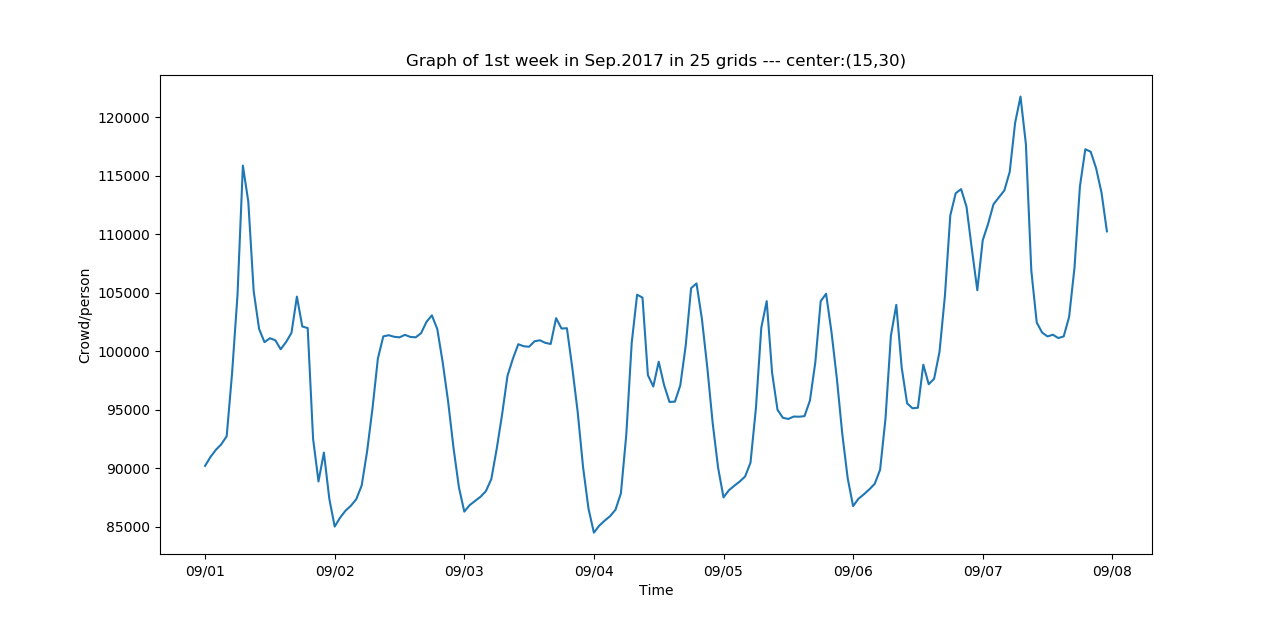
\includegraphics[width=0.8\textwidth]{month9_week1_25grids.png}
\caption{25个网格内人流一周内变化}
\label{fig:2.2}
\end{figure}
之所以取25个网格观察,是希望弱化网格间人口流量的影响,主要观察时序变化规律。
\indent 可以发现:
\begin{enumerate}
	\item 每天的人口驻留数量有明显的周期性变化。凌晨左右的人口数量最低。
	\item 已知09/02和09/03是周末,发现周末的人口数据与周中人口数据有所不同。
\end{enumerate}
\subsubsection*{人流变化的长周期性}
观察以(15,30)为中心25个网格的三周内人口数量变化,图(\ref{fig:2.3})中红线代表每周周六,可以看到人口数量在各周间也有所波动。
\begin{figure}[ht]
\centering
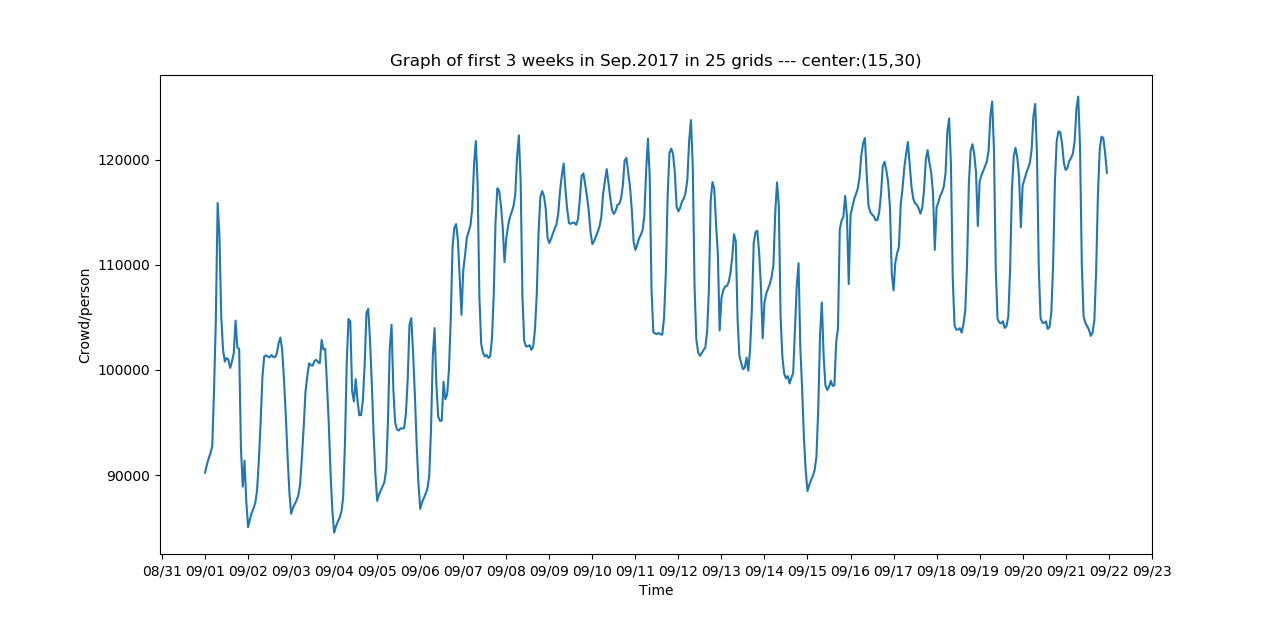
\includegraphics[width=0.8\textwidth]{month9_week3_25grids.png}
\caption{25个网格内人流三周内变化}
\label{fig:2.3}
\end{figure}
\subsubsection*{相邻地域的关联性}
以(15,30)(15,31)两个网格一天的人口流动为例,可以观测网格位置关联的地域的人流相关性。
\begin{figure}[ht]
\centering
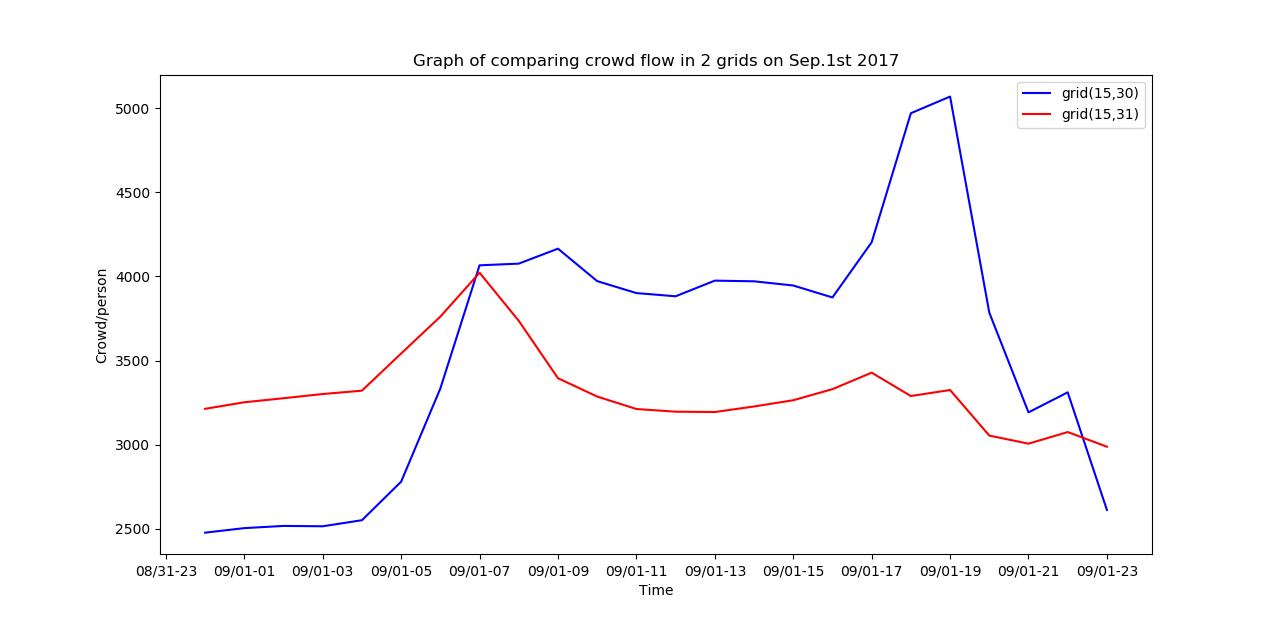
\includegraphics[width=0.8\textwidth]{compare.png}
\caption{两个相邻网格一天的人口流动}
\label{fig:2.4}
\end{figure}
从图(\ref{fig:2.4})中,
观察绿色框,可以发现一个网格人口增多另一个网格人口减少,其原因可能与人们在这两地移动相关,这在一定程度上体现网格位置对人口流动的影响。
\subsubsection*{天气和节假日的影响}
天气和节假日都可能对人流产生影响,也应该成为预测中的一个重要因素。以中关村区域为例,如图(\ref{fig:weather})所示,区域的中雨使得和周期性的规律相比人流有所下降;而如图(\ref{fig:holiday})所示,在十一假期间,该的确的人流有了和普通工作日相比显著的减小。
\begin{figure}[ht]
\centering
\subfloat[十一假期对于人流变化的影响]{\label{fig:weather}{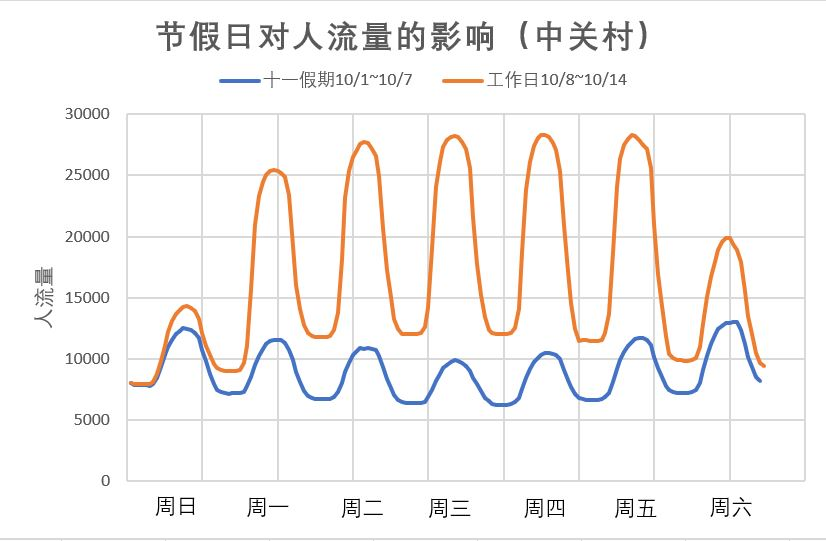
\includegraphics[width=0.45\textwidth]{holiday.jpg}}}
\subfloat[天气对于人流变化的影响]{\label{fig:holiday}{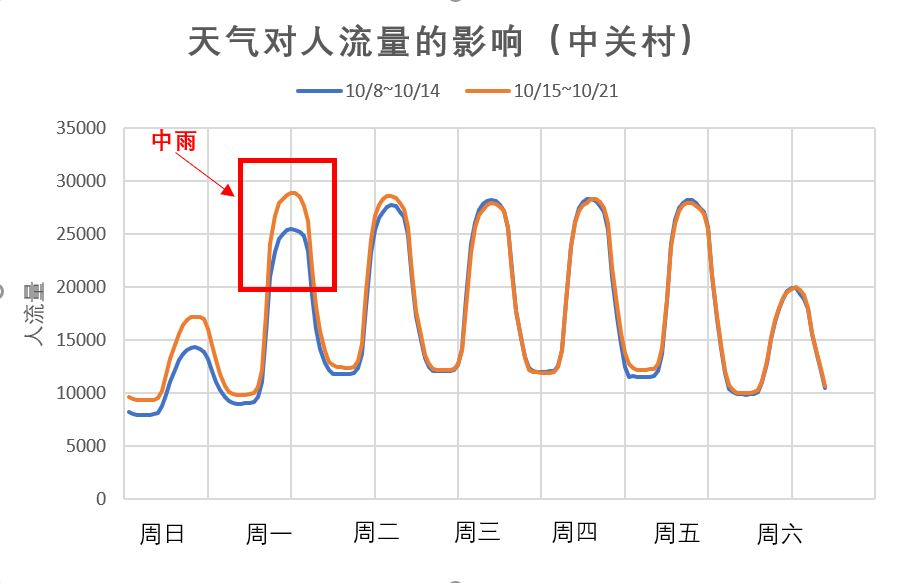
\includegraphics[width=0.45\textwidth]{weather.jpg}}}
\hfill
\caption{节假日和天气因素对于人口流动的影响:以中关村为例}
%\label{fig:subfigures}
\end{figure}
在我们的模型中,也可以很方便的对于这两个外部因素加以考量,只需要在之前的模型中加入额外的天气和节假日的维度即可,用数学公式可以表达为
\begin{equation}
\bar{\mu_i} = \mu_i + \psi_{i,w_t}+\theta_{i,h_t}
\end{equation}
其中 $\mu_i$ 为原始的向量,而$\psi_{i,w_t}$和$\theta_{i,h_t}$分别为天气和假期的影响
\\
基于以上对于数据的清洗和对于数据特征和规律的初步分析,我们得到了在实际的预测分析需要考察的主要影响因素:
\begin{itemize}
	\item 时间上的周期性变化,又分为近期、中期和较长期的影响,需要在模型中进行不同权重的影响的分配
	\item 空间上的互相影响,诸如城市功能区、道路、特别是邻近区块的互相影响,需要在模型中仔细加以考量
	\item 天气和节假日等特殊因素的影响,也需要在模型中加以体现
\end{itemize}
\section{技术方案选择}
\subsection{可选技术方案}
\subsubsection*{ARIMA时序数据预测方法}
\label{arima}
对于非平稳的时序序列,常常可以采用差分自回归移动平均模型(Autoregressive–moving-average model,ARIMA)进行分析\cite{whittle1966prediction,Hannan1970Multiple}。
在ARIMA(p,d,q)模型中,p 代表自回归阶数,d 代表差分次数, q 代表移动平均阶数,这一模型的建立需要解决以下三个问题:
\begin{enumerate}
	\item 利用差分将非平稳序列转化为平稳序列
	\item 通过模式识别确定模型属于AR、MA、ARMA中的哪一种
	\item 通过模式识别确定模型属于AR、MA、ARMA中的哪一种
\end{enumerate}
\indent 基于此,一种简单的预测方式可以对每个网格的时序序列进行建模求解,得到初步的预测情况。但是,网格的数量有两千两百多个,求解的计算量是较大的。同时,这样一来便没有考虑网格的位置分布关系对人口流动的影响。\\
\indent 基于这一模型的特点,比较适用于对于一些感兴趣的网络进行初步近似求解。
\subsubsection*{Res-CNN方法}
有文献\cite{Zhang2016Deep}指出,对于试图预测的某一时刻人口数量,在时序上,受到3个部分的影响:
\begin{itemize}
	\item $X_c$邻近时刻(例如之前的几个小时)
	\item $X_p$周期(例如昨天、前天的同一时刻)
	\item $X_q$趋势(例如上周、上上周等的同一时刻)
\end{itemize}
所以可以利用相同的网络结构来处理以上三部分信息。
\indent 另外,由于卷积层CNN通过卷积核的扫描融入了网格分布的位置信息,多个卷积层的叠加又可以使特征层次有小到大,所以文章先利用CNN对信息进行处理。
为了改善卷积层过深梯度消失的问题,在卷积层后加入了残差网络Res\ref{fig:2.5},从而构成了时序部分的网络结构。

\begin{figure}[ht]
\centering
\subfloat[卷积层和残差单元]{\label{fig:2.5}{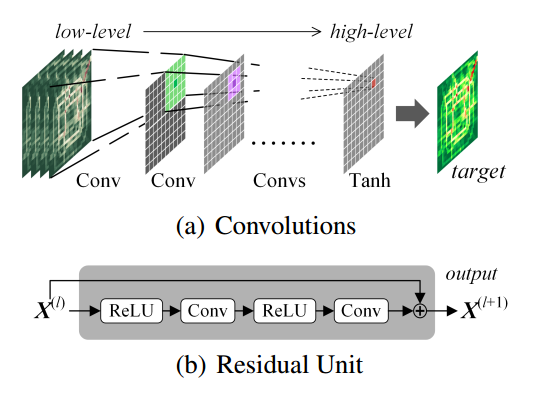
\includegraphics[width=0.45\textwidth]{Residual.png}}}
\subfloat[网络结构]{\label{fig:2.6}{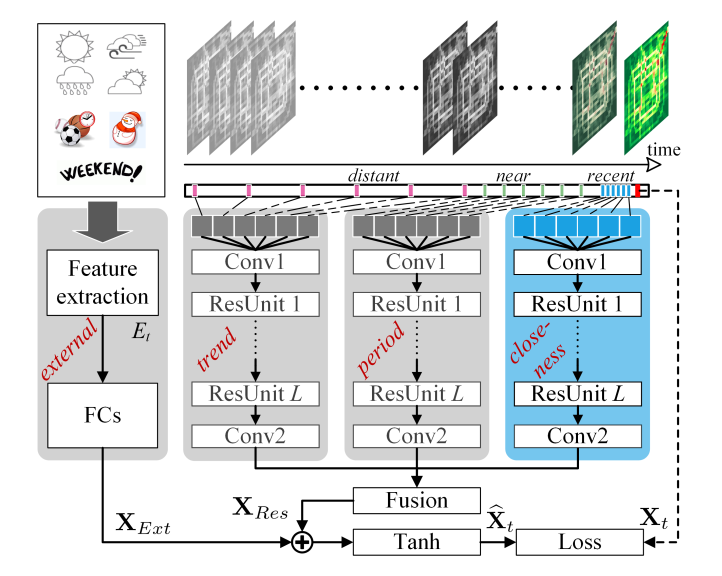
\includegraphics[width=0.45\textwidth]{net.png}}}
\hfill
\caption{残差网络结构}
%\label{fig:subfigures}
\end{figure}
最后,三个相同结构网络得到的数据,通过与参数矩阵相乘再相加的方式进行融合与维度的统一。同时训练得到了矩阵中的参数。
\\
\indent 另外,还可以考虑外部因素$E_t$(如天气等)对于人口流动的影响,其最终的网络结构如图(\ref{fig:2.6})所示。
其中左侧是处理外部因素的,右侧是3个相似的卷积残差网络用来处理时序数据。将$E_t$转变成对应的特征向量,在其后连接两个全连接层FC。第一个全连接层可以看作对特征的提取,第二层则是为了获得与时序数据处理结果有相同维度。两部分最后的融合方式直接相加,并通过双曲正切函数控制在(-1,1)之间。网络的损失函数为预测与实际值误差的平方:
\begin{equation}
Loss = \Arrowvert y_t - \hat{y_t} \Arrowvert^2
\end{equation}
